% Texto integral do artigo, carregado diretamente dos arquivos originais.
% Padrão visual: MTC Modelo de Apresentação oral do projet de pesquisa.pdf.
% Compilação: make slides (pdfLaTeX + BibTeX, via latexmk).
\documentclass[aspectratio=169,10pt,t]{beamer}

\usepackage[utf8]{inputenc}
\usepackage[T1]{fontenc}
\usepackage[brazilian]{babel}
\usepackage{helvet,courier,mathptmx}
\usepackage{graphicx,array,ragged2e,colortbl}
\usepackage[alf,abnt-emphasize=bf,bibjustif,recuo=0cm,
  abnt-etal-cite=3,abnt-etal-list=0,abnt-etal-text=it]{abntex2cite}

% Uma única coluna, sem barras, rodapés, numeração de slides ou ornamentos.
% As medidas reproduzem proporcionalmente a fonte Arial 20 pt e as margens
% do modelo de 960 x 540 pt no tamanho nativo 16:9 do Beamer.
\usetheme{default}
\usefonttheme{professionalfonts}
\setbeamersize{text margin left=1.05cm,text margin right=1.05cm}
\setbeamercolor{normal text}{fg=black,bg=white}
\setbeamercolor{structure}{fg=black}
\setbeamercolor{bibliography entry author}{fg=black}
\setbeamercolor{bibliography entry title}{fg=black}
\setbeamercolor{bibliography entry location}{fg=black}
\setbeamercolor{bibliography entry note}{fg=black}
\setbeamerfont{normal text}{size*={9.5}{11.35}}
\setbeamerfont{itemize/enumerate body}{size*={9.5}{11.35}}
\setbeamerfont{caption}{size*={8}{9.6}}
\setbeamerfont{caption name}{size*={8}{9.6}}
\setbeamerfont{quote}{shape=\upshape}
\setbeamerfont{bibliography entry author}{size*={9.5}{11.35}}
\setbeamerfont{bibliography entry title}{size*={9.5}{11.35}}
\setbeamerfont{bibliography entry location}{size*={9.5}{11.35}}
\setbeamerfont{bibliography entry note}{size*={9.5}{11.35}}
\setbeamertemplate{navigation symbols}{}
\setbeamertemplate{headline}{\vspace{0.6cm}}
\setbeamertemplate{footline}{\vspace{0.45cm}}
\setbeamertemplate{frametitle}{}
\setbeamertemplate{frametitle continuation}{}
\setbeamertemplate{bibliography item}{}
\setbeamertemplate{caption}[numbered]
\setbeamertemplate{itemize item}{\raisebox{0.15ex}{\scriptsize\textbullet}}
\urlstyle{same}
\hypersetup{colorlinks=true,linkcolor=black,citecolor=black,urlcolor=blue,
  pdfsubject={Texto integral do projeto de pesquisa — IFCE Campus Maracanaú}}
\title{Raciocínio Lógico em LLMs: Avaliação de Processos Dedutivos na Resolução de Sudoku}
\author{João Pedro Moreira Campos de Lima; Isaac da Cunha Cavalcanti Duarte; Juliano Magalhães Jurity}
\date{2026}

% Adaptação apenas dos comandos de apresentação do artigo. O conteúdo dos
% capítulos não é copiado, reescrito, resumido ou convertido em novos tópicos.
\newcounter{capituloartigo}
\newcounter{secaoartigo}[capituloartigo]
\newcounter{subsecaoartigo}[secaoartigo]
\newcommand{\tituloartigo}[1]{%
  \par\refstepcounter{capituloartigo}%
  \noindent\textbf{\arabic{capituloartigo}\space\MakeUppercase{#1}}\par
  \nobreak\vspace{6pt}\nobreak}
\newcommand{\chapter}[1]{\tituloartigo{#1}}
\newcommand{\secaoprimariasemquebra}[1]{\tituloartigo{#1}}
\newcommand{\apendice}[1]{%
  \par\noindent\textbf{APÊNDICE A — \MakeUppercase{#1}}\par
  \nobreak\vspace{6pt}\nobreak}
\newenvironment{alineascomponto}{%
  \begin{itemize}\setlength{\itemsep}{0pt}\setlength{\parsep}{0pt}}{\end{itemize}}
\newcommand{\Caption}[1]{\caption{#1}}
\newcommand{\Fonte}[1]{\par{\fontsize{8}{9.6}\selectfont Fonte: #1\par}}
\let\imagemoriginal\includegraphics

\newenvironment{conteudointegral}{%
  \usebeamerfont{normal text}\justifying
  \setlength{\parindent}{0pt}\setlength{\parskip}{2pt}%
  % Evita separar as linhas de um parágrafo entre slides.
  \interlinepenalty=10000\widowpenalty=10000\clubpenalty=10000
  \renewcommand{\section}[1]{%
    \par\addvspace{6pt}\refstepcounter{secaoartigo}%
    \noindent\textbf{\arabic{capituloartigo}.\arabic{secaoartigo}\space ##1}\par\nobreak}%
  \renewcommand{\subsection}[1]{%
    \par\addvspace{6pt}\refstepcounter{subsecaoartigo}%
    \noindent\textbf{\arabic{capituloartigo}.\arabic{secaoartigo}.\arabic{subsecaoartigo}\space ##1}\par\nobreak}%
  % Conserva todas as figuras; limita apenas sua altura para caber no slide.
  \renewcommand{\includegraphics}[2][]{%
    \imagemoriginal[##1,height=0.64\textheight,keepaspectratio]{##2}}%
}{\par}

\newsavebox{\tabelacronograma}
\let\tabularoriginal\tabular
\let\fimtabularoriginal\endtabular
\let\pilhaoriginal\shortstack
\newcommand{\ajustartabela}{%
  \renewcommand{\shortstack}[1]{\cellcolor{yellow}\pilhaoriginal{##1}}%
  \renewenvironment{tabular}[1]{%
    \begin{lrbox}{\tabelacronograma}\tabularoriginal{##1}%
  }{%
    \fimtabularoriginal\end{lrbox}%
    \resizebox{0.93\linewidth}{!}{\usebox{\tabelacronograma}}%
  }}

\begin{document}

% Capa: logotipo, instituição, título serifado, autores e orientadora,
% centralizados, na mesma ordem do modelo. Sem informações adicionais.
\begin{frame}[plain]
  \centering
  \vspace{0.35cm}
  \imagemoriginal[height=1.75cm]{figuras/logo-ifce.png}\par
  \vspace{0.05cm}
  {\fontsize{9.5}{11.35}\selectfont IFCE Campus Maracanaú\\Ciência da Computação\par}
  \vspace{0.14cm}
  {\fontfamily{ptm}\selectfont\fontsize{15.1}{16.2}\selectfont
    RACIOCÍNIO LÓGICO EM LLMs:\\
    AVALIAÇÃO DE PROCESSOS DEDUTIVOS\\
    NA RESOLUÇÃO DE SUDOKU\par}
  \vspace{0.28cm}
  {\fontsize{9.5}{11.35}\selectfont
    João Pedro Moreira Campos de Lima\\
    Isaac da Cunha Cavalcanti Duarte\\
    Juliano Magalhães Jurity\par}
  \vspace{0.15cm}
  {\fontsize{9.5}{11.35}\selectfont
    Orientadora: Profa. Ma. Aurenívia Ferreira da Silva\par}
\end{frame}

% Cada bloco pode continuar em novas páginas. A ordem e todo o conteúdo
% são os dos mesmos arquivos incluídos por documento.tex.
\begin{frame}[allowframebreaks=1]
  \begin{conteudointegral}
    \chapter{Introdução}

\section{Delimitação do tema}

Modelos de Linguagem de Grande Escala, ou LLMs, são sistemas capazes de ler e produzir textos. Eles costumam responder de forma fluida e convincente, mas uma explicação bem escrita não garante que o raciocínio apresentado esteja correto. Esta pesquisa investiga essa diferença em uma tarefa simples de conferir: encontrar e explicar uma única jogada de Sudoku.

O Sudoku foi escolhido porque suas regras são objetivas. Uma pessoa ou um programa pode verificar se uma jogada respeita a linha, a coluna e o bloco da célula. Isso permite observar duas coisas separadamente: se a LLM chegou ao valor certo e se a explicação que ela deu realmente justifica esse valor.

Assim, este estudo trabalhará com Sudokus 4 $\times$ 4 e 9 $\times$ 9. O tabuleiro começa com algumas células preenchidas, chamadas pistas, e outras vazias. O objetivo é preencher as células vazias sem alterar as pistas. Em cada linha, coluna e bloco, cada número permitido deve aparecer uma única vez. No Sudoku 4 $\times$ 4, usam-se os números de 1 a 4 e os blocos têm 2 $\times$ 2 células. No Sudoku 9 $\times$ 9, usam-se os números de 1 a 9 e os blocos têm 3 $\times$ 3 células.

\begin{figure}[!ht]
\centering
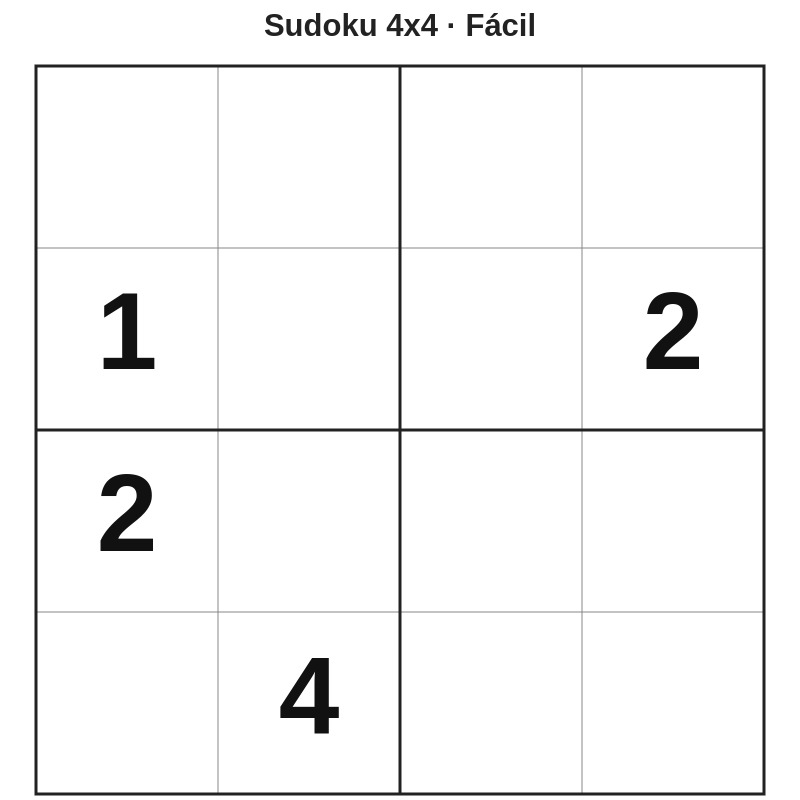
\includegraphics[width=0.62\textwidth]{figuras/sudoku-4x4-easy}
\Caption{Exemplo de tabuleiro Sudoku 4 $\times$ 4\label{fig:intro-sudoku}}
\Fonte{EducColorir (s.d.). Disponível em: \url{https://www.educolorir.com/gerador-de-sudoku}. Acesso em: 21 out. 2026.}
\end{figure}

Para indicar uma posição, o texto usa a forma L$\mathit{x}$C$\mathit{y}$, em que L significa linha e C significa coluna. A contagem começa em 1. Assim, L1C4 é a célula da primeira linha e da quarta coluna. Essa é uma notação pensada para leitura humana; mais adiante, a metodologia mostra como a mesma posição aparece no programa.

Uma célula vazia pode receber apenas números que não estejam em sua linha, coluna ou bloco. Esses números possíveis são chamados de candidatos. Se, em um Sudoku 4 $\times$ 4, uma célula não pode receber 1, 2 ou 4, resta apenas o número 3. A partir dessa ideia, a pesquisa analisa três maneiras de encontrar uma jogada.

No \textit{Naked Single}, uma célula fica com apenas um candidato. No \textit{Hidden Single}, um número pode continuar sendo candidato em mais de uma célula do tabuleiro, mas só pode aparecer em uma posição de uma linha, coluna ou bloco. No consenso de primeira camada, o programa considera hipóteses temporárias, acompanha o que acontece em cada uma e procura uma conclusão que se repete em todos os caminhos possíveis.

O recorte do estudo é uma jogada por vez e somente essas três técnicas. A intenção não é afirmar como uma LLM funciona internamente. O objetivo é verificar se ela produz uma jogada válida e se a explicação apresentada combina com a técnica solicitada.

\section{Problematização}

Quando uma LLM apresenta uma resposta convincente, é fácil assumir que ela raciocinou corretamente. Em tarefas lógicas, porém, ela pode acertar o valor por outro caminho, usar uma técnica diferente da pedida ou escrever uma justificativa que não sustenta a conclusão. Avaliar apenas a resposta final deixa esses casos escondidos.

O Sudoku cria um ambiente controlado para observar esse problema. As regras são claras, a jogada pode ser conferida automaticamente e a dificuldade pode ser ajustada. As técnicas de \textit{Naked Single} e \textit{Hidden Single} dependem apenas das informações visíveis no tabuleiro. O consenso exige que a LLM acompanhe hipóteses e compare as consequências de cada uma.

Diante disso, a pesquisa busca responder: como as LLMs se comportam ao indicar e justificar uma jogada de Sudoku que exige uma dedução direta ou uma comparação entre hipóteses?

\section{Hipótese}

Espera-se que as LLMs tenham melhor desempenho em \textit{Naked Single} e \textit{Hidden Single}, pois essas técnicas dependem de restrições visíveis na grade. No consenso, espera-se mais dificuldade, porque a tarefa exige manter hipóteses temporárias, acompanhar suas consequências e encontrar uma conclusão comum.

\section{Justificativa}

Avaliar LLMs com Sudoku ajuda a separar duas coisas que frequentemente aparecem misturadas: acertar uma resposta e explicar bem por que ela está certa. Como cada jogada pode ser conferida por regras objetivas, o estudo permite identificar respostas corretas com justificativas fracas, justificativas coerentes que chegam a uma conclusão errada e respostas que seguem exatamente a técnica solicitada.

Os resultados podem contribuir para avaliações de sistemas que precisam explicar suas decisões em linguagem clara. O estudo também oferece um conjunto de critérios simples para examinar respostas de LLMs em tarefas estruturadas, nas quais é possível conferir tanto o resultado quanto o caminho usado para chegar a ele.

  \end{conteudointegral}
\end{frame}

\begin{frame}[allowframebreaks=1]
  \begin{conteudointegral}
    \secaoprimariasemquebra{Objetivos}

\section{Objetivo geral}

\begin{alineascomponto}
\item Avaliar a capacidade de LLMs para indicar e justificar uma jogada em Sudokus 4 $\times$ 4 e 9 $\times$ 9 que exija dedução direta ou raciocínio por hipóteses.
\end{alineascomponto}

\section{Objetivos específicos}

\begin{alineascomponto}
\item Organizar e validar instâncias de Sudoku classificadas como \textit{Naked Single}, \textit{Hidden Single} ou consenso de primeira camada;
\item Submeter as mesmas instâncias aos modelos selecionados, com instruções e configurações padronizadas, registrando a identificação do modelo, a configuração usada e a resposta original;
\item Verificar se a jogada indicada é aceita pelo verificador da técnica solicitada;
\item Analisar se a justificativa apresentada corresponde às evidências exigidas em cada técnica;
\item Comparar o desempenho dos modelos entre deduções diretas e raciocínio por hipóteses.
\end{alineascomponto}

  \end{conteudointegral}
\end{frame}

\begin{frame}[allowframebreaks=1]
  \begin{conteudointegral}
    \secaoprimariasemquebra{Referencial teórico}

Esta seção apresenta as ideias usadas para construir e avaliar o experimento. Primeiro, explica por que uma resposta correta não é suficiente para avaliar uma LLM. Depois, mostra como o Sudoku permite conferir cada passo da resolução e apresenta as três técnicas usadas na pesquisa.

\section{Raciocínio lógico e respostas de LLMs}

Neste trabalho, raciocinar significa usar informações e regras para chegar a uma conclusão. Para fazer isso, é preciso observar o que já se sabe, comparar possibilidades e descartar aquelas que entram em conflito com as regras. \citeonline{dagostino2024} discutem como esse processo pode ser limitado pelos recursos disponíveis para quem raciocina.

Uma LLM pode escrever uma explicação clara e, ainda assim, apresentar uma conclusão que não decorre das informações fornecidas. No benchmark TruthQuest, \citeonline{mondorf2024} observam dificuldades dos modelos ao lidar com hipóteses e com as consequências de premissas possivelmente falsas. Por isso, nesta pesquisa, a explicação será observada junto com a jogada final, e não como uma prova automática de que o modelo raciocinou corretamente.

Alguns problemas exigem explorar caminhos alternativos antes de decidir. \citeonline{herr2025} investigam esse tipo de busca em LLMs e mostram que ela pode ajudar em tarefas estruturadas, como Sudoku. O consenso de primeira camada usa essa ideia de forma limitada: o programa cria hipóteses simples, acompanha suas consequências e só aceita uma conclusão quando ela aparece em todos os caminhos viáveis.

\section{Sudoku como problema de restrições}

O Sudoku também pode ser visto como um problema de satisfação de restrições. Esse nome descreve problemas em que valores precisam ser escolhidos sem quebrar regras. No Sudoku, cada célula é uma posição que deve receber um número. As pistas já têm valores definidos; as células vazias precisam ser preenchidas. As regras de linha, coluna e bloco limitam quais números podem ser usados.

Em uma grade 9 $\times$ 9, por exemplo, cada linha, cada coluna e cada bloco de 3 $\times$ 3 deve conter os números de 1 a 9 uma única vez. Resolver o tabuleiro significa encontrar valores para as células vazias que respeitem todas essas regras ao mesmo tempo. Essa estrutura é útil para a pesquisa porque permite verificar se uma jogada é válida sem depender de opinião humana.

\begin{figure}[!ht]
\centering
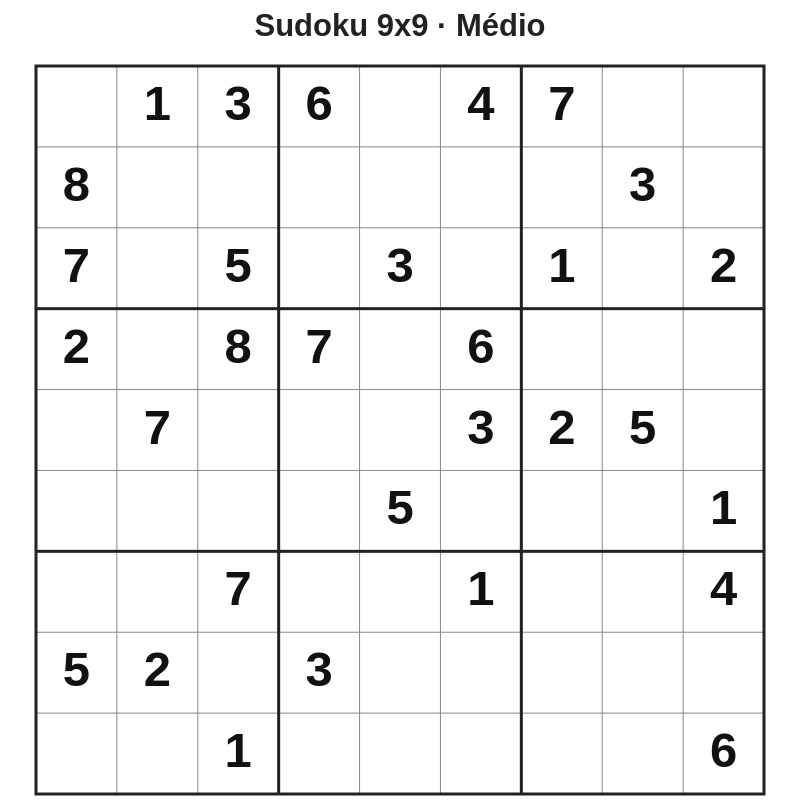
\includegraphics[width=0.72\textwidth]{figuras/sudoku-9x9-medium}
\Caption{Exemplo de tabuleiro Sudoku 9 $\times$ 9\label{fig:tabuleiro-sudoku}}
\Fonte{EducColorir (s.d.). Disponível em: \url{https://www.educolorir.com/gerador-de-sudoku}. Acesso em: 21 out. 2026.}
\end{figure}

\citeonline{sudokuSage2026} usam o Sudoku para avaliar jogadas individuais propostas por LLMs. A quantidade e a distribuição das pistas alteram a dificuldade do tabuleiro, enquanto as regras permitem conferir a jogada com precisão. Essas duas características tornam o Sudoku adequado para o experimento.

\subsection{Como as técnicas são identificadas}

Nas Figuras \ref{fig:naked-single}, \ref{fig:hidden-single} e \ref{fig:consenso-sudoku}, L e C significam linha e coluna, com contagem iniciada em 1. Portanto, L2C3 é a célula da segunda linha e da terceira coluna. A expressão $C(\text{L2C3})$ representa os candidatos dessa célula. Uma unidade é uma linha, uma coluna ou um bloco.

Um candidato é um número que ainda não foi eliminado pelas regras. Ele não é uma resposta confirmada; ele apenas continua possível naquele momento. As três técnicas usadas no estudo partem desse conjunto de possibilidades.

No \textit{Naked Single}, a análise é feita em uma célula: se há um único candidato, esse valor é a jogada. Na Figura \ref{fig:naked-single}, a célula L1C4 está vazia. A linha 1 já contém 2, 4 e 1; a coluna 4 já contém 4, 1 e 2; e o bloco superior direito já contém 1, 2 e 4. Assim, todos os valores, exceto 3, são eliminados. Como $C(\text{L1C4})=\{3\}$, L1C4 recebe 3.

\begin{figure}[!ht]
\centering
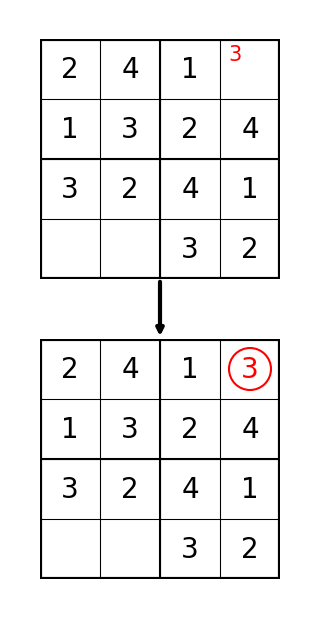
\includegraphics[width=0.45\textwidth]{figuras/instancia-1-naked-single}
\Caption{Instância 1 do conjunto de dados: aplicação de \textit{Naked Single}\label{fig:naked-single}}
\Fonte{Dados da pesquisa (2026).}
\end{figure}

No \textit{Hidden Single}, a análise é feita em uma unidade inteira. Na Figura \ref{fig:hidden-single}, a linha 2 tem três células vazias. L2C1 e L2C4 têm candidatos $\{1,3\}$, enquanto L2C2 tem $\{1,3,4\}$. A célula L2C2 não é um \textit{Naked Single}, pois tem três candidatos. Mesmo assim, o número 4 só aparece como possibilidade em L2C2 nessa linha. Como a linha precisa conter o número 4, L2C2 deve receber 4.

\begin{figure}[!ht]
\centering
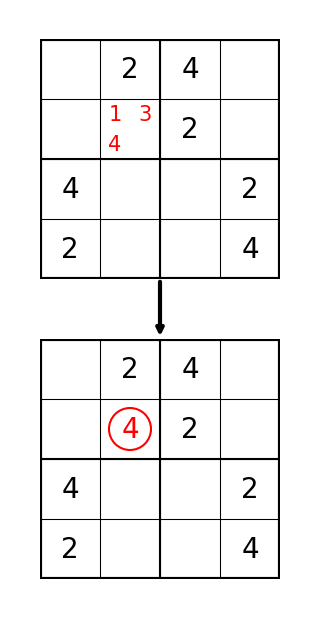
\includegraphics[width=0.45\textwidth]{figuras/instancia-160-hidden-single}
\Caption{Instância 160 do conjunto de dados: aplicação de \textit{Hidden Single}\label{fig:hidden-single}}
\Fonte{Dados da pesquisa (2026).}
\end{figure}

O consenso é usado quando não há uma dedução direta disponível. O programa escolhe um número que pode ocupar mais de uma posição em uma unidade. Cada posição possível cria uma versão provisória da grade, chamada de ramo. Em cada ramo, o programa aplica apenas \textit{Naked Singles} e \textit{Hidden Singles}. Se todos os ramos que respeitam as regras levam ao mesmo valor em uma célula, essa conclusão pode ser usada no tabuleiro original.

Na Figura \ref{fig:consenso-sudoku}, o número 3 da primeira linha pode ficar em L1C1 ou em L1C4. O primeiro ramo supõe que L1C1 recebe 3; o segundo supõe que L1C4 recebe 3. Depois das deduções diretas, os dois ramos concluem que L1C2 recebe 2. Como o resultado é o mesmo nos dois casos, o programa insere 2 em L1C2 sem precisar escolher qual hipótese inicial é a verdadeira.

\begin{figure}[!ht]
\centering
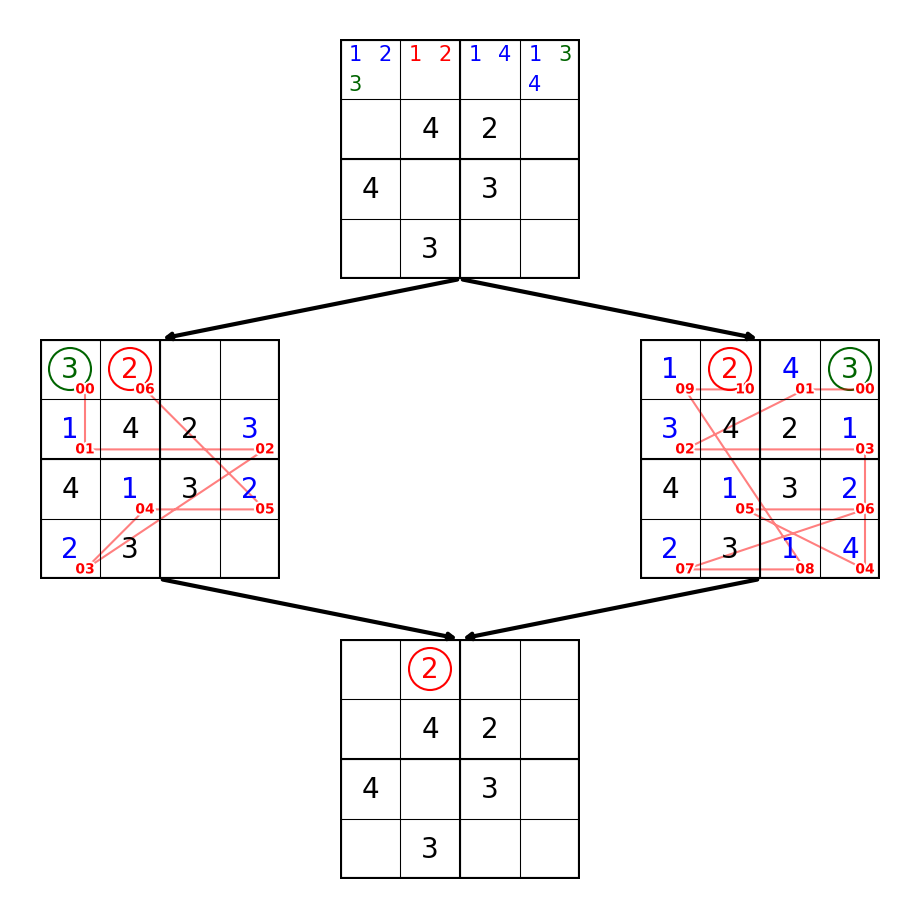
\includegraphics[width=0.9\textwidth]{figuras/instancia-301-consensus}
\Caption{Instância 301 do conjunto de dados: aplicação do consenso de primeira camada\label{fig:consenso-sudoku}}
\Fonte{Dados da pesquisa (2026).}
\end{figure}

\section{Avaliação das respostas e das explicações}

A avaliação se compõe de duas partes. A primeira é automática: o programa confere se a posição e o valor indicados pela LLM correspondem a uma jogada aceita para a técnica solicitada. A segunda examina se a justificativa apresentada usa as informações necessárias para sustentar a jogada.

Para \textit{Naked Single}, a explicação precisa mostrar por que só resta um candidato na célula. Para \textit{Hidden Single}, ela precisa indicar a linha, coluna ou bloco analisado e mostrar que o valor só cabe em uma posição. Para consenso, precisa apresentar as hipóteses, as deduções feitas em cada ramo e a conclusão comum. \citeonline{maiya2025} mostram que uma solução correta não garante uma explicação que represente adequadamente a estratégia usada.

Ao comparar as três técnicas, a pesquisa verifica se a correção da jogada e a qualidade da explicação mudam quando a tarefa passa de uma dedução direta para uma comparação entre hipóteses. Os resultados mostram se a resposta é compatível com regras e procedimentos definidos previamente; eles não são usados para afirmar, de forma direta, como o modelo funciona internamente.

  \end{conteudointegral}
\end{frame}

\begin{frame}[allowframebreaks=1]
  \begin{conteudointegral}
    \secaoprimariasemquebra{Metodologia}

Esta pesquisa seguirá uma sequência simples. Primeiro, o programa criará tabuleiros e identificará a técnica presente em cada um. Depois, uma LLM receberá esses tabuleiros e proporá uma jogada. Por fim, o programa conferirá a jogada e a explicação. O código do experimento será disponibilizado em repositório público. Uma base piloto será usada para testar o processo e orientar a etapa comparativa da pesquisa.

O experimento usará Sudokus 4 $\times$ 4 e 9 $\times$ 9. Dentro do programa, uma célula vazia será representada por zero. Os demais números serão as pistas do tabuleiro. Por exemplo, a posição que o leitor vê como L1C4 aparecerá no programa como $[0,3]$: o programa começará a contar linhas e colunas a partir de zero, enquanto o texto começará em 1.

A seguir, serão apresentadas as etapas a serem seguidas.

\section{Como o programa lerá o tabuleiro}

O tabuleiro será guardado como uma matriz, isto é, uma lista de linhas. Em um Sudoku 4 $\times$ 4, haverá quatro linhas, quatro colunas e blocos de 2 $\times$ 2 células. Em um Sudoku 9 $\times$ 9, haverá nove linhas, nove colunas e blocos de 3 $\times$ 3 células.

Para cada célula vazia, o programa começará com todos os números permitidos. Em seguida, removerá os números que aparecerem na linha, na coluna e no bloco da célula. Os números restantes formarão o conjunto de candidatos. A partir desse conjunto, o programa reconhecerá as técnicas que serão usadas no estudo.

Em termos formais, se $x$ for uma célula vazia e $V_n=\{1,2,\ldots,n\}$ for o conjunto de números permitidos, os candidatos serão calculados por:

\[
\operatorname{Cand}_G(x)=V_n\setminus\bigl(L(x)\cup C(x)\cup B(x)\bigr).
\]

Na fórmula, $L(x)$ reunirá os números presentes na linha de $x$, $C(x)$ os números da coluna e $B(x)$ os números do bloco. O símbolo $\setminus$ indicará a retirada de elementos de um conjunto. A fórmula, portanto, expressará o procedimento descrito no parágrafo anterior: começar com todos os números e excluir os que não poderão ser usados.

O \textit{Naked Single} será identificado quando a célula ficar com um único candidato:

\[
\left|\operatorname{Cand}_G(x)\right|=1.
\]

O \textit{Hidden Single} será identificado quando um número $v$ só puder ser colocado em uma célula de uma unidade $U$, sendo $U$ uma linha, coluna ou bloco:

\[
\left|\left\{x\in U : v\in\operatorname{Cand}_G(x)\right\}\right|=1.
\]

Para o consenso de primeira camada, o programa escolherá um número que tenha mais de uma posição possível em uma mesma unidade. Cada possibilidade criará um ramo, ou seja, uma cópia temporária do tabuleiro. Dentro de cada ramo, o programa aplicará apenas \textit{Naked Singles} e \textit{Hidden Singles}. Se todos os ramos viáveis chegarem ao mesmo valor para uma célula alvo, esse valor será aceito no tabuleiro original. Em linguagem lógica, se $D(G_p)(t)=a$ em todos os ramos viáveis $p$, então a célula alvo $t$ receberá $a$:

\[
\forall p\in P_v^{\mathrm{viaveis}},\quad D(G_p)(t)=a
\quad\Longrightarrow\quad t=a.
\]

Aqui, $P_v^{\mathrm{viaveis}}$ representará as posições que ainda forem possíveis para o valor $v$. A expressão $D(G_p)$ representará a grade depois das deduções diretas feitas no ramo $p$. A expressão ``primeira camada'' indicará que o programa não criará uma nova hipótese dentro do ramo: ele apenas acompanhará as consequências da hipótese inicial.

\section{Como o Z3 verificará as grades}

Além de calcular candidatos, o programa usará o Z3, um solucionador de restrições lógicas. Para o Z3, cada célula será uma variável inteira entre 1 e $n$. Ele receberá três regras: os valores de uma linha não poderão se repetir, os valores de uma coluna não poderão se repetir e os valores de um bloco não poderão se repetir. As pistas existentes também ficarão fixadas aos seus valores.

A formalização a seguir escreverá essas mesmas regras em símbolos. Ela acompanhará diretamente o que o código entregará ao Z3: primeiro as regras da grade, depois as pistas e, por fim, a busca pelas soluções possíveis.

\subsection{Modelo lógico que será usado pelo Z3}

Para tornar essa etapa precisa, seja $x_{ij}$ a variável que será criada para a célula da linha $i$ e da coluna $j$. O código criará uma variável para cada célula, inclusive para as pistas. Em uma grade de ordem $n$, as restrições de domínio serão:

\[
1 \leq x_{ij} \leq n,
\qquad 0 \leq i,j < n.
\]

Em seguida, o Z3 receberá uma restrição de valores distintos para cada linha, cada coluna e cada bloco. Se $q=\sqrt{n}$ for o tamanho do lado de um bloco, essa parte do modelo poderá ser escrita como:

\[
\begin{aligned}
&\operatorname{Distinct}(x_{i0},x_{i1},\ldots,x_{i,n-1}) && \text{para toda linha } i;\\
&\operatorname{Distinct}(x_{0j},x_{1j},\ldots,x_{n-1,j}) && \text{para toda coluna } j;\\
&\operatorname{Distinct}\bigl(\{x_{rq+a,\,sq+b}:0\leq a,b<q\}\bigr) && \text{para cada bloco } (r,s).
\end{aligned}
\]

A última linha representará os blocos: $r$ e $s$ indicarão em qual bloco a célula estará, enquanto $a$ e $b$ indicarão sua posição dentro dele. Por exemplo, em um Sudoku 9 $\times$ 9, $q=3$; cada bloco terá três linhas e três colunas. O termo \textit{Distinct} indicará que os valores listados deverão ser diferentes entre si.

Se a entrada do tabuleiro possuir uma pista $g_{ij}$ diferente de zero, o código fixará a variável correspondente:

\[
g_{ij}\neq 0 \quad \Longrightarrow \quad x_{ij}=g_{ij}.
\]

O conjunto formado por todas essas restrições será chamado de $\Phi_G$. Uma solução do Sudoku será qualquer preenchimento que respeite $\Phi_G$. Para uma posição, o programa reunirá os valores que aparecerem nessa posição ao percorrer todas as soluções encontradas. Se aparecer apenas um valor, a posição será globalmente forçada; se aparecerem dois ou mais valores, a posição continuará admitindo mais de uma possibilidade. Essa noção será usada pelo código ao preencher os campos de validação da resposta da LLM. A escrita formal desse conjunto estará no Apêndice A.

O Z3 procurará um preenchimento completo que respeite todas essas regras. Quando encontrar uma solução, o programa adicionará uma nova regra que obrigará a próxima solução a ser diferente dela em pelo menos uma célula. Repetindo esse procedimento, o programa identificará se a grade será insatisfatível, terá uma solução única ou admitirá mais de uma solução.

Mais exatamente, se $M_k$ for a $k$-ésima solução obtida, o código adicionará a restrição de bloqueio:

\[
\beta_k=\bigvee_{0\leq i,j<n}\bigl(x_{ij}\neq M_k(x_{ij})\bigr).
\]

Essa expressão obrigará a próxima solução a discordar de $M_k$ em pelo menos uma célula. Depois de encontrar $k$ soluções, o Z3 procurará uma nova solução para $\Phi_G\land\beta_1\land\cdots\land\beta_k$. O símbolo $\land$ indicará a conjunção entre as restrições: o Z3 precisará respeitar as regras do Sudoku e todas as restrições de bloqueio que tiverem sido criadas. Quando essa busca se tornar insatisfatível, todas as soluções da grade terão sido enumeradas.

Essa etapa não substituirá a classificação das técnicas. O detector de técnicas responderá à pergunta ``qual jogada poderá ser obtida ao se observar a grade?''. O Z3 responderá a outra pergunta: ``quais valores aparecerão em soluções completas compatíveis com esta grade?''. Essa diferença será importante quando a resposta da LLM for avaliada.

\section{Construção do conjunto de dados}

O conjunto de dados será formado a partir de grades completas a serem obtidas com o Z3. O programa escolherá uma grade que terá sido resolvida, embaralhará suas posições e removerá pistas uma a uma. A solução de origem continuará compatível com o tabuleiro reduzido, pois a remoção de uma pista não alterará os valores que compõem a solução. Depois de cada remoção, o programa recalculará os candidatos e verificará se a técnica desejada terá aparecido.

As categorias serão separadas para que cada instância cubra a técnica esperada. Uma instância de \textit{Hidden Single} só será guardada quando não houver \textit{Naked Single} disponível. Uma instância de consenso só será guardada quando não houver nenhuma das duas deduções diretas. Para \textit{Naked Single}, o programa esperará que pelo menos 25\% das células tenham sido removidas e também descartará grades que já tenham \textit{Hidden Single} disponível.

O processo não exigirá solução única para guardar uma instância. Isso será intencional: o programa registrará se a jogada sugerida pela LLM será o único valor possível ou se será compatível com pelo menos uma solução. Para cada instância, o banco de dados guardará a grade, a técnica identificada e uma imagem do tabuleiro. Para cada inferência, guardará a explicação escrita pela LLM e os resultados da validação.

\section{Envio para a LLM e avaliação das respostas}

Cada instância será enviada à LLM como texto. O comando informará a grade, explicará que zero representará célula vazia, indicará a técnica que deverá ser usada e pedirá uma única jogada. Quando houver mais de uma jogada possível, o comando pedirá a célula com menor índice de linha e, em caso de empate, a de menor índice de coluna. Essa regra tornará a escolha reprodutível.

A resposta deverá ser apresentada em JSON, um formato de texto organizado por campos, com o valor proposto, a posição da célula, a técnica usada e a explicação da jogada. O exemplo a seguir ilustra esse formato para uma jogada de \textit{Naked Single}:

\begin{quote}
\small\ttfamily
\{\par
\quad "value": 3,\par
\quad "position": [0, 3],\par
\quad "candidate\_type": "ZEROTH\_LAYER\_NAKED\_SINGLES",\par
\quad "explanation": "O valor 3 é o único candidato da célula."\par
\}
\end{quote}

A avaliação automática considerará três critérios. O primeiro será a adequação à técnica solicitada: o programa verificará se a posição e o valor propostos corresponderão a uma das jogadas identificadas pelo detector dessa técnica. O segundo será a compatibilidade com as soluções da grade: o Z3 verificará se haverá pelo menos uma solução completa em que a célula indicada contenha o valor proposto. O terceiro será a obrigatoriedade desse valor na posição escolhida: será verificado se todas as soluções completas apresentarão o mesmo valor nessa célula.

Esses critérios permitirão distinguir uma jogada que respeite a técnica pedida de uma proposta que seja apenas compatível com alguma solução da grade. Também permitirão identificar se o valor será obrigatório naquela célula ou se outras soluções admitirão valores diferentes para a mesma posição. Caso o valor proposto não apareça em nenhuma solução, a jogada será considerada incompatível com a grade. A explicação da LLM será preservada para a análise do raciocínio apresentado.

Depois da conferência automática, o pesquisador lerá a explicação com uma rubrica simples. Em \textit{Naked Single}, verificará se ela identificará a célula e mostrará por que os demais valores terão sido eliminados. Em \textit{Hidden Single}, verificará se ela apontará a linha, coluna ou bloco analisado e mostrará por que o valor só caberá em uma posição. Em consenso, verificará se ela apresentará as hipóteses, relatará as deduções de cada ramo e explicará a conclusão comum. Para cada item, o pesquisador registrará a presença, a incompletude ou a ausência da evidência. A mesma rubrica será aplicada a todas as respostas, para que os critérios permaneçam consistentes.

Na etapa piloto, será realizada uma inferência por instância. Cada execução registrará o modelo, sua versão, os parâmetros adotados, a data da chamada, o JSON completo retornado pela LLM, a explicação e os resultados da validação. Na etapa comparativa, as mesmas instâncias serão submetidas aos modelos selecionados com comandos padronizados. Com esses registros, será possível comparar as taxas de acerto e a qualidade das justificativas entre modelos e entre as três técnicas.

  \end{conteudointegral}
\end{frame}

\begin{frame}
  \begin{conteudointegral}
    % Mantém a tabela original inteira, ajustando sua largura à página.
    \ajustartabela
    \chapter{Cronograma}

\begin{center}
\small
\setlength{\tabcolsep}{2pt}
\renewcommand{\arraystretch}{1.35}
\begin{tabular}{|p{5.5cm}|*{8}{>{\centering\arraybackslash}p{1.05cm}|}}
\hline
\textbf{Etapas/atividades} & \shortstack{\textbf{Set.}\\\textbf{2026}} & \shortstack{\textbf{Out.}\\\textbf{2026}} & \shortstack{\textbf{Nov.}\\\textbf{2026}} & \shortstack{\textbf{Dez.}\\\textbf{2026}} & \shortstack{\textbf{Jan.}\\\textbf{2027}} & \shortstack{\textbf{Fev.}\\\textbf{2027}} & \shortstack{\textbf{Mar.}\\\textbf{2027}} & \shortstack{\textbf{Abr.}\\\textbf{2027}} \\
\hline
Levantamento bibliográfico & X & & & & & & & \\
\hline
Seleção, fichamento e resenha dos textos & X & X & & & & & & \\
\hline
Organização da fundamentação teórica & & X & & & & & & \\
\hline
Análise crítica dos materiais & & X & X & & & & & \\
\hline
Escrita da fundamentação teórica & & & X & X & & & & \\
\hline
Descrição da metodologia & & & & X & & & & \\
\hline
Discussão dos resultados & & & & & X & X & & \\
\hline
Revisão e redação final & & & & & & & X & \\
\hline
Defesa da pesquisa & & & & & & & & X \\
\hline
\end{tabular}
\end{center}

  \end{conteudointegral}
\end{frame}

\nocite{dagostino2024,sudokuSage2026,herr2025,maiya2025,mondorf2024}
\begin{frame}[allowframebreaks=1]
  \begin{conteudointegral}
    \textbf{REFERÊNCIAS}\par\vspace{11.35pt}
    \bibliography{elementos-pos-textuais/referencias}
  \end{conteudointegral}
\end{frame}

% O apêndice também integra o artigo e é preservado integralmente.
\begin{frame}[allowframebreaks=1]
  \begin{conteudointegral}
    \apendice{Formalização complementar das soluções do Sudoku}

Este apêndice reúne a parte mais abstrata da formalização do Z3. Ela detalha a ideia apresentada na metodologia: o programa enumera soluções completas para descobrir quais valores continuam possíveis em cada célula.

Seja $\Phi_G$ o conjunto de restrições de uma grade $G$. Uma solução completa é uma atribuição $M$ de valores às células que satisfaz todas essas restrições. O conjunto de soluções é:

\[
\operatorname{Sol}(G)=\{M : M\models\Phi_G\}.
\]

Nessa expressão, $M\models\Phi_G$ significa que o preenchimento $M$ respeita as regras da grade, as pistas e as restrições de linha, coluna e bloco.

Para uma célula localizada na posição $[i,j]$, os valores que aparecem entre todas as soluções completas são definidos por:

\[
\operatorname{Poss}_G(i,j)=\{M(x_{ij}) : M\in\operatorname{Sol}(G)\}.
\]

Se $\left|\operatorname{Poss}_G(i,j)\right|=1$, apenas um valor aparece naquela posição e a célula é globalmente forçada pela grade. Se $\left|\operatorname{Poss}_G(i,j)\right|>1$, mais de um valor pode ocupar a posição em soluções diferentes. O código usa essa distinção ao avaliar se a jogada proposta pela LLM é apenas compatível com alguma solução ou se é única naquela célula.

  \end{conteudointegral}
\end{frame}

\end{document}
